\documentclass[journal,10pt,twocolumn]{IEEEtran}

\usepackage{amsmath,amssymb,amsfonts}
\usepackage{algorithmic}
\usepackage{graphicx}
\usepackage{textcomp}
\usepackage{xcolor}
\usepackage{booktabs}
\usepackage{cite}
\usepackage{bm}
\usepackage{siunitx}
\usepackage{subcaption}

\begin{document}

\title{A High-Fidelity Multi-Physics Benchmark for Industrial Robot Motion Control Under Varying Payloads, Multi-Rate Inverter Dynamics, and Reflected Actuator Inertia}

\author{Robotics and Advanced Control Research Group%
\thanks{Manuscript received November 1, 2026. This work was supported by the Department of Electrical and Electronics Engineering, Ton Duc Thang University.}%
}

\maketitle

\begin{abstract}
Trajectory tracking control of multi-degree-of-freedom (DOF) industrial manipulators subjected to abrupt payload variations remains a foundational challenge in robotics. In the overwhelming majority of robotics literature, motion controllers are evaluated under idealized kinematic torque sources ($\bm{\tau}_{\text{motor}} \equiv \bm{\tau}_{\text{cmd}}$), ignoring the electromechanical dynamics of permanent magnet synchronous motor (PMSM) drives, discrete field-oriented current control (FOC) latencies, space-vector pulse-width modulation (SVPWM) circular voltage clipping ($V_{dc}/\sqrt{3}$), and dynamic DC-link voltage fluctuations. Furthermore, the immense contribution of reflected actuator rotor inertia ($N^2 J_m$), which can exceed bare link inertia by over $1,500\times$, is almost universally omitted in standard multi-body formulations.

In this work, we establish an end-to-end, physically grounded cyber-physical benchmarking pipeline for the 6-DOF Unimation PUMA 560 manipulator. Physical parameters are calibrated directly against the authoritative experimental identification benchmarks of Armstrong et al. (1988) and Corke (1996). We comprehensively evaluate four control paradigms: (i) Gravity Compensation + Proportional-Derivative (PD), (ii) Feedback Linearizing Computed Torque Control (CTC), (iii) Nonlinear PID (NPID) with adaptive state-dependent gain scheduling, and (iv) Linear Active Disturbance Rejection Control (LADRC) equipped with a 3rd-order Linear Extended State Observer (LESO).

The evaluation is conducted across three rigorous simulation scenarios: (1) Standard Pick-and-Place Benchmark (9.20s cycle) with an unmodeled dynamic payload step ($0 \to 3.5\,\text{kg} \to 0\,\text{kg}$), where LADRC achieves an 87.2\% reduction in ISE ($4.34\,\text{deg}^2\cdot\text{s}$ vs. $33.97\,\text{deg}^2\cdot\text{s}$ for CTC) and suppresses shoulder static droop down to $0.23^\circ$ RMS; (2) High-Speed Aggressive Benchmark (3.07s duration, $3\times$ speed scaling) evaluating back-EMF headroom and SVPWM voltage circle saturation; and (3) Parametric Sensitivity Stress Test ($+20\%$ unmodeled link mass and inertia mismatch across all joints), proving that while CTC degrades severely by $+62.9\%$ in ISE and $+74.6\%$ in IAE, LADRC demonstrates near-invariant tracking (only $+6.3\%$ degradation).
\end{abstract}

\begin{IEEEkeywords}
Industrial Manipulators, PUMA 560, Active Disturbance Rejection Control, Computed Torque Control, Reflected Actuator Inertia, Multi-Rate Inverter, Parametric Sensitivity, Shared DC Bus.
\end{IEEEkeywords}

\section{Introduction}
\IEEEPARstart{H}{igh}-speed pick-and-place manipulation constitutes the cornerstone of modern manufacturing, packaging, and robotic assembly \cite{craig2005introduction}. In such operations, articulated manipulators must follow high-order smooth trajectories while experiencing discontinuous changes in link mass and inertia tensors at the grasping and releasing instants.

Classic trajectory tracking formulations assume torque is generated instantaneously by ideal actuators \cite{spong2020robot}. However, in commercial robotics, torque is produced by high-frequency inverter-fed motors, typically Permanent Magnet Synchronous Motors (PMSM) equipped with high-ratio gear reducers (e.g., Harmonic Drives) and powered by a regulated shared direct current (DC) link capacitor bus \cite{siciliano2008springer}. When a heavy payload is acquired, not only do the mechanical equations of motion change instantaneously, but the motor current demands surge, causing voltage sag on the DC link, dead-time voltage distortion across inverter legs, and sudden saturation of inner current control loops.

While advanced robust and adaptive controllers have been widely proposed in theoretical literature \cite{slotine1991applied, gao2003scaling}, industrial deployments continue to predominantly rely on decentralized PD/PID controllers or nominal feedback linearization. Therefore, there is a distinct necessity for a rigorous, standardized, multi-physics benchmark that quantifies both tracking performance metrics (ISE, IAE, ITAE, RMSE, Peak Error) and electro-mechanical energy consumption when subject to unmodeled dynamic payloads.

This paper provides the following contributions:
\begin{enumerate}
    \item \textbf{Cyber-Physical Modeling Grounded in Experimental Benchmarks:} Calibration of link masses, inertia tensors, and friction coefficients directly against the experimentally identified PUMA 560 parameters of Armstrong et al. \cite{armstrong1988experimental} and Corke \cite{corke1996robot}.
    \item \textbf{Actuator Reflected Inertia Dominance:} Proof that geared rotor inertia $N^2 J_m$ exceeds bare link inertia by over $1,500\times$ in the wrist axes, proving that drive-level inertia inclusion is indispensable for physical accuracy.
    \item \textbf{Discrete Multi-Rate Inverter Dynamics:} Coupling mechanical multi-body dynamics ($500\,\text{Hz}$ RK4) with discrete $10\,\text{kHz}$ field-oriented current control in the $d$-$q$ rotating frame, 1-step DSP calculation delay ($z^{-1}$), inverter dead-time ($t_d = 1.2\,\mu\text{s}$) with active compensation, and dynamic DC-link voltage droop with finite SMPS closed-loop response.
    \item \textbf{Comprehensive Multi-Scenario Benchmark Suite:} Systematic comparative evaluation across three distinct stress scenarios: (1) Standard Nominal Trajectory, (2) High-Speed Aggressive Motion with Space Vector voltage saturation ($V_{dc}/\sqrt{3} \approx 27.7\,\text{V}$), and (3) $+20\%$ Parametric Sensitivity Stress Test proving robust stability without requiring physical arm disassembly.
\end{enumerate}

\section{Cyber-Physical System Modeling}

\subsection{Rigid-Body Manipulator Dynamics with Reflected Actuator Inertia}
The equation of motion of an $n$-degree-of-freedom manipulator subjected to an end-effector payload and geared motor drives is expressed in joint space:
\begin{equation}
    \bm{M}(\bm{q}, m_p, \bm{J}_{\text{refl}})\ddot{\bm{q}} + \bm{C}(\bm{q}, \dot{\bm{q}}, m_p)\dot{\bm{q}} + \bm{g}(\bm{q}, m_p) + \bm{F}_v \dot{\bm{q}} = \bm{\tau}
    \label{eq:manipulator_dynamics}
\end{equation}
where $\bm{q}, \dot{\bm{q}}, \ddot{\bm{q}} \in \mathbb{R}^n$ denote the generalized joint position, velocity, and acceleration vectors; $\bm{M} \in \mathbb{R}^{n \times n}$ is the generalized inertia matrix:
\begin{equation}
    \bm{M}(\bm{q}, m_p, \bm{J}_{\text{refl}}) = \bm{M}_{\text{rigid}}(\bm{q}, m_p) + \text{diag}\left(N_j^2 J_{m,j}\right)
\end{equation}
where $N_j$ is the transmission gear ratio and $J_{m,j}$ is the motor rotor inertia. $\bm{C}(\bm{q}, \dot{\bm{q}}, m_p) \in \mathbb{R}^{n \times n}$ contains Coriolis and centripetal terms satisfying $\dot{\bm{M}} - 2\bm{C} = -(\dot{\bm{M}} - 2\bm{C})^T$; $\bm{g}(\bm{q}, m_p) \in \mathbb{R}^n$ represents gravitational generalized forces; $\bm{F}_v \in \mathbb{R}^{n \times n}$ is the joint viscous friction diagonal matrix; and $\bm{\tau} \in \mathbb{R}^n$ is the joint actuation torque vector delivered by the transmission.

In our framework, all inertial parameters ($m_j, \bm{c}_j, \bm{I}_j$) are calibrated strictly against the experimental identification logs of Armstrong et al. \cite{armstrong1988experimental} and Corke \cite{corke1996robot}. The actuators follow authentic industrial frameless PMSM sizing:
\begin{itemize}
    \item Joint 1 (Waist): RoboDrive ILM 70x18 ($N_1 = 62.61, J_m = 2.0\times 10^{-4}\,\text{kg}\cdot\text{m}^2$).
    \item Joint 2 (Shoulder): RoboDrive ILM 70x18 HD ($N_2 = 107.83, J_m = 2.0\times 10^{-4}\,\text{kg}\cdot\text{m}^2$).
    \item Joint 3 (Elbow): RoboDrive ILM 70x10 ($N_3 = 53.71, J_m = 1.3\times 10^{-4}\,\text{kg}\cdot\text{m}^2$).
    \item Joint 4--5 (Wrist): RoboDrive ILM 38x10 ($N = 75.91, 71.92, J_m = 3.3\times 10^{-5}\,\text{kg}\cdot\text{m}^2$).
    \item Joint 6 (Flange): RoboDrive ILM 38x06 ($N_6 = 76.69, J_m = 1.7\times 10^{-5}\,\text{kg}\cdot\text{m}^2$).
\end{itemize}
For Joint 4, the reflected rotor inertia is:
\begin{equation}
    J_{\text{refl},4} = N_4^2 J_{m,4} = 75.91^2 \times (3.3\times 10^{-5}) = 0.190\,\text{kg}\cdot\text{m}^2
\end{equation}
which is \textbf{$1,580\times$ larger} than the bare rigid link inertia ($I_{xx,4} = 0.00012\,\text{kg}\cdot\text{m}^2$). Omitting reflected inertia leads to catastrophic underestimation of required motor torque.

The dynamic payload $m_p(t)$ picked at $t = 3.5\,\text{s}$ and released at $t = 7.5\,\text{s}$ modifies the mass and spatial inertia tensor of the 6th link:
\begin{equation}
    m_p(t) = 
    \begin{cases}
        0\,\text{kg}, & t < 3.5\,\text{s} \\
        3.5\,\text{kg}, & 3.5\,\text{s} \le t \le 7.5\,\text{s} \\
        0\,\text{kg}, & t > 7.5\,\text{s}
    \end{cases}
\end{equation}

\subsection{Multi-Rate PMSM Actuator and Discrete Field-Oriented Control}
Each joint is driven by a multi-rate discrete Field-Oriented Controlled (FOC) drive executing in the rotating $d$-$q$ reference frame. Inner current control operates at high frequency ($10\,\text{kHz}$, $\Delta t_{\text{sub}} = 100\,\mu\text{s}$) with discrete PI controllers tuned for pole-zero cancellation:
\begin{align}
    v_q^*(k) &= K_{pq}(i_q^*(k-1) - i_q(k)) + K_{iq} \sum (i_q^* - i_q)\Delta t_{\text{sub}} \nonumber \\
    &\quad + 0.95 \omega_e (L_d i_d + \lambda_{\text{PM}}) + v_{q,\text{dead}} \\
    v_d^*(k) &= K_{pd}(0 - i_d(k)) + K_{id} \sum (0 - i_d)\Delta t_{\text{sub}} \nonumber \\
    &\quad - 0.95 \omega_e L_q i_q + v_{d,\text{dead}}
\end{align}
where:
\begin{itemize}
    \item $i_q^*(k-1)$ models real-world 1-step DSP computation and ADC sampling latency.
    \item A 5\% parameter uncertainty in cross-coupling decoupling injects authentic transient interactions between $d$ and $q$ axes.
    \item Inverter dead-time ($t_d = 1.2\,\mu\text{s}$, $f_{sw} = 16\,\text{kHz}$) with active digital feedforward (92\% cancellation) leaves residual 6th harmonic distortion:
    \begin{equation}
        v_{q,\text{dead}} = -0.08 \cdot \left(\frac{4}{\pi} \frac{t_d}{T_{sw}} V_{dc}\right) \text{sgn}(i_q) \cos(6\theta_e)
    \end{equation}
    \item Space Vector PWM enforces the circular linear modulation ceiling:
    \begin{equation}
        \sqrt{v_d^{*2} + v_q^{*2}} \le \frac{V_{dc}}{\sqrt{3}} \approx 27.7\,\text{V} \quad (\text{for } V_{dc} = 48\,\text{V})
    \end{equation}
\end{itemize}

Physical stator phase dynamics are integrated via:
\begin{align}
    \frac{di_d}{dt} &= \frac{1}{L_d}(v_d - R_s i_d + \omega_e L_q i_q) \\
    \frac{di_q}{dt} &= \frac{1}{L_q}(v_q - R_s i_q - \omega_e(L_d i_d + \lambda_{\text{PM}}))
\end{align}
Electromagnetic torque delivered to the motor shaft is $\tau_m = K_t \cdot i_q$, and torque delivered to the arm link is:
\begin{equation}
    \tau_j = (\tau_m - B_m \dot{\theta}_m) N_j \eta_j
\end{equation}

\subsection{Power Inverter and Shared DC Bus Capacitor Dynamics}
All 6 inverters are connected to a common DC link capacitor $C_{\text{bus}} = 4700\,\mu\text{F}$ ($R_{\text{ESR}} = 15\,\text{m}\Omega$) supplied by an industrial Switched-Mode Power Supply (SMPS) with finite regulation response ($\tau_{\text{ps}} = 8\,\text{ms}$) and internal droop impedance ($R_{\text{ps}} = 60\,\text{m}\Omega$):
\begin{equation}
    C_{\text{bus}} \frac{dV_{dc}}{dt} = I_{\text{supply}}(t) - \sum_{j=1}^6 I_{\text{inv},j}(t) - I_{\text{brake}}(t)
\end{equation}
where $I_{\text{inv},j} = P_{\text{elec},j} / V_{dc}$. During deceleration, regenerative power elevates $V_{dc}$. When $V_{dc} \ge 56.0\,\text{V}$, a dynamic braking chopper with a $4.7\,\Omega$ resistor dissipates excess energy:
\begin{equation}
    I_{\text{brake}} = \frac{V_{dc}}{R_{\text{brake}}}
\end{equation}

\section{Trajectory Tracking Controllers}

\subsection{Controller 1: Gravity Compensation + PD}
Gravity Compensation + PD utilizes a feedforward gravity cancellation based on nominal kinematics and uncoupled joint feedback:
\begin{equation}
    \bm{\tau}_{\text{ctrl}} = \hat{\bm{g}}(\bm{q}) + \bm{K}_p \bm{e} + \bm{K}_d \dot{\bm{e}}
\end{equation}
where $\bm{e} = \bm{q}_d - \bm{q}$, $\dot{\bm{e}} = \dot{\bm{q}}_d - \dot{\bm{q}}$, and $\bm{K}_p, \bm{K}_d > 0$ are constant diagonal matrices. By Lyapunov stability analysis, asymptotic regulation is guaranteed under nominal models. However, when an unmodeled payload is engaged, steady-state position droop manifests as:
\begin{equation}
    \bm{e}_{ss} = \bm{K}_p^{-1} \Delta \bm{g}(\bm{q})
\end{equation}

\subsection{Controller 2: Computed Torque Control (CTC)}
Computed Torque Control employs inverse dynamics feedback linearization:
\begin{equation}
    \bm{\tau}_{\text{ctrl}} = \hat{\bm{M}}(\bm{q}) \left( \ddot{\bm{q}}_d + \bm{K}_v \dot{\bm{e}} + \bm{K}_p \bm{e} \right) + \hat{\bm{C}}(\bm{q}, \dot{\bm{q}})\dot{\bm{q}} + \hat{\bm{g}}(\bm{q})
\end{equation}
Under ideal parameters ($\hat{\bm{M}} = \bm{M}$, $\hat{\bm{C}} = \bm{C}$, $\hat{\bm{g}} = \bm{g}$), the closed loop decouples into $n$ independent linear second-order error systems. However, under unmodeled payload disturbance $\Delta \bm{M}$ and $\Delta \bm{g}$, the true error dynamics become perturbed:
\begin{equation}
    \ddot{\bm{e}} + \bm{K}_v \dot{\bm{e}} + \bm{K}_p \bm{e} = \bm{M}^{-1} \left( \Delta \bm{M} \ddot{\bm{q}} + \Delta \bm{C} \dot{\bm{q}} + \Delta \bm{g} \right)
\end{equation}
which induces high transient degradation during acceleration phases.

\subsection{Controller 3: Nonlinear PID (NPID)}
To counter gravitational droop while maintaining compliant operation during nominal motion, an adaptive Nonlinear PID architecture is formulated:
\begin{equation}
    \bm{\tau}_{\text{ctrl}} = \hat{\bm{g}}(\bm{q}) + \bm{K}_p(\bm{e}) \bm{e} + \bm{K}_d \dot{\bm{e}} + \bm{K}_i \int_0^t \bm{e}(\sigma) d\sigma
\end{equation}
where the proportional gain is dynamically scheduled according to instantaneous tracking error:
\begin{equation}
    K_{p,j}(e_j) = K_{p0,j} \left[ 1 + \alpha_j \tanh(\beta_j e_j^2) \right]
\end{equation}
Here, $K_{p0,j}$ is baseline stiffness, $\alpha_j > 0$ determines the maximum stiffness gain multiplier, and $\beta_j > 0$ controls transition steepness.

\subsection{Controller 4: Linear Active Disturbance Rejection Control (LADRC)}
Each joint is modeled as a perturbed second-order motion subsystem \cite{gao2003scaling}:
\begin{equation}
    \ddot{q}_j = b_{0, j} \tau_j + f_j(q, \dot{q}, \ddot{q}_d, \tau_{\text{load}}, t)
\end{equation}
where $b_{0, j} = 1 / (J_{\text{refl}, j} + M_{jj}(q))$, and $f_j$ represents the total generalized disturbance aggregating Coriolis torques, gravity, payload steps, dead-time harmonics, and parameter mismatches. A 3rd-order Linear Extended State Observer (LESO) estimates the state vector $[z_1, z_2, z_3]^T \approx [q_j, \dot{q}_j, f_j]^T$:
\begin{align}
    \dot{z}_{1, j} &= z_{2, j} + 3\omega_o (q_j - z_{1, j}) \\
    \dot{z}_{2, j} &= z_{3, j} + b_{0, j} \tau_j + 3\omega_o^2 (q_j - z_{1, j}) \\
    \dot{z}_{3, j} &= \omega_o^3 (q_j - z_{1, j})
\end{align}
with observer bandwidth $\omega_o = 120\,\text{rad/s}$. The control law cancels the estimated disturbance in real time:
\begin{equation}
    \tau_j = \frac{k_p (q_{d, j} - z_{1, j}) + k_d (\dot{q}_{d, j} - z_{2, j}) + \ddot{q}_{d, j} - z_{3, j}}{b_{0, j}}
\end{equation}
where $k_p = \omega_c^2$, $k_d = 2\omega_c$, and controller bandwidth $\omega_c = 40\,\text{rad/s}$.

\section{Quantitative Benchmark Results}

The benchmark was executed across three distinct experimental simulation scenarios.

\subsection{Scenario 1: Standard Pick-and-Place Benchmark (9.20s Cycle)}
Table~\ref{tab:scenario1_results} summarizes the performance across 4,601 integration steps ($\Delta t = 2.0\,\text{ms}$) under an unmodeled 3.5 kg payload.

\begin{table*}[t]
\centering
\caption{Scenario 1: Standard Trajectory Benchmark Performance (Duration: 9.20s, Nominal Model, 3.5 kg Payload)}
\label{tab:scenario1_results}
\begin{tabular}{lcccc}
\toprule
\textbf{Evaluation Metric} & \textbf{[1] Gravity Comp + PD} & \textbf{[2] Computed Torque (CTC)} & \textbf{[3] Nonlinear PID (NPID)} & \textbf{[4] Linear ADRC (LESO)} \\
\midrule
\textbf{Total ISE ($\text{deg}^2\cdot\text{s}$)} & 103.39 & 33.97 & 46.84 & \textbf{4.34} \\
\textbf{Total IAE ($\text{deg}\cdot\text{s}$)}   & 31.64 & 18.76 & 21.68 & \textbf{5.36} \\
\textbf{Total ITAE ($\text{deg}\cdot\text{s}^2$)} & 161.08 & 92.62 & 108.71 & \textbf{25.21} \\
RMS Error Joint 1 ($^\circ$) & 0.3515 & 0.3064 & 0.2445 & \textbf{0.0853} \\
RMS Error Joint 2 ($^\circ$) & 1.4655 & 1.0237 & 0.9989 & \textbf{0.2316} \\
RMS Error Joint 3 ($^\circ$) & 0.4045 & 0.4189 & 0.2841 & \textbf{0.1262} \\
RMS Error Joint 4 ($^\circ$) & 2.9652 & 1.5408 & 1.9866 & \textbf{0.6276} \\
RMS Error Joint 5 ($^\circ$) & 0.0719 & \textbf{0.0169} & 0.0568 & 0.0217 \\
RMS Error Joint 6 ($^\circ$) & 0.0559 & \textbf{0.0140} & 0.0473 & 0.0209 \\
\midrule
\textbf{Peak Joint Torque ($\text{N}\cdot\text{m}$)} & 85.6 & 85.2 & 85.3 & \textbf{84.7} \\
\textbf{Total Net Electrical Energy} & 72.7 J (0.020 Wh) & 72.3 J (0.020 Wh) & 72.0 J (0.020 Wh) & \textbf{70.7 J (0.020 Wh)} \\
\textbf{Regenerated Braking Energy} & 116.5 J & 113.1 J & 114.6 J & \textbf{110.2 J} \\
\textbf{DC Bus Voltage Swing} & 47.5V -- 48.6V & 47.5V -- 48.6V & 47.5V -- 48.6V & 47.5V -- 48.6V \\
\bottomrule
\end{tabular}
\end{table*}

\begin{figure}[t]
\centering
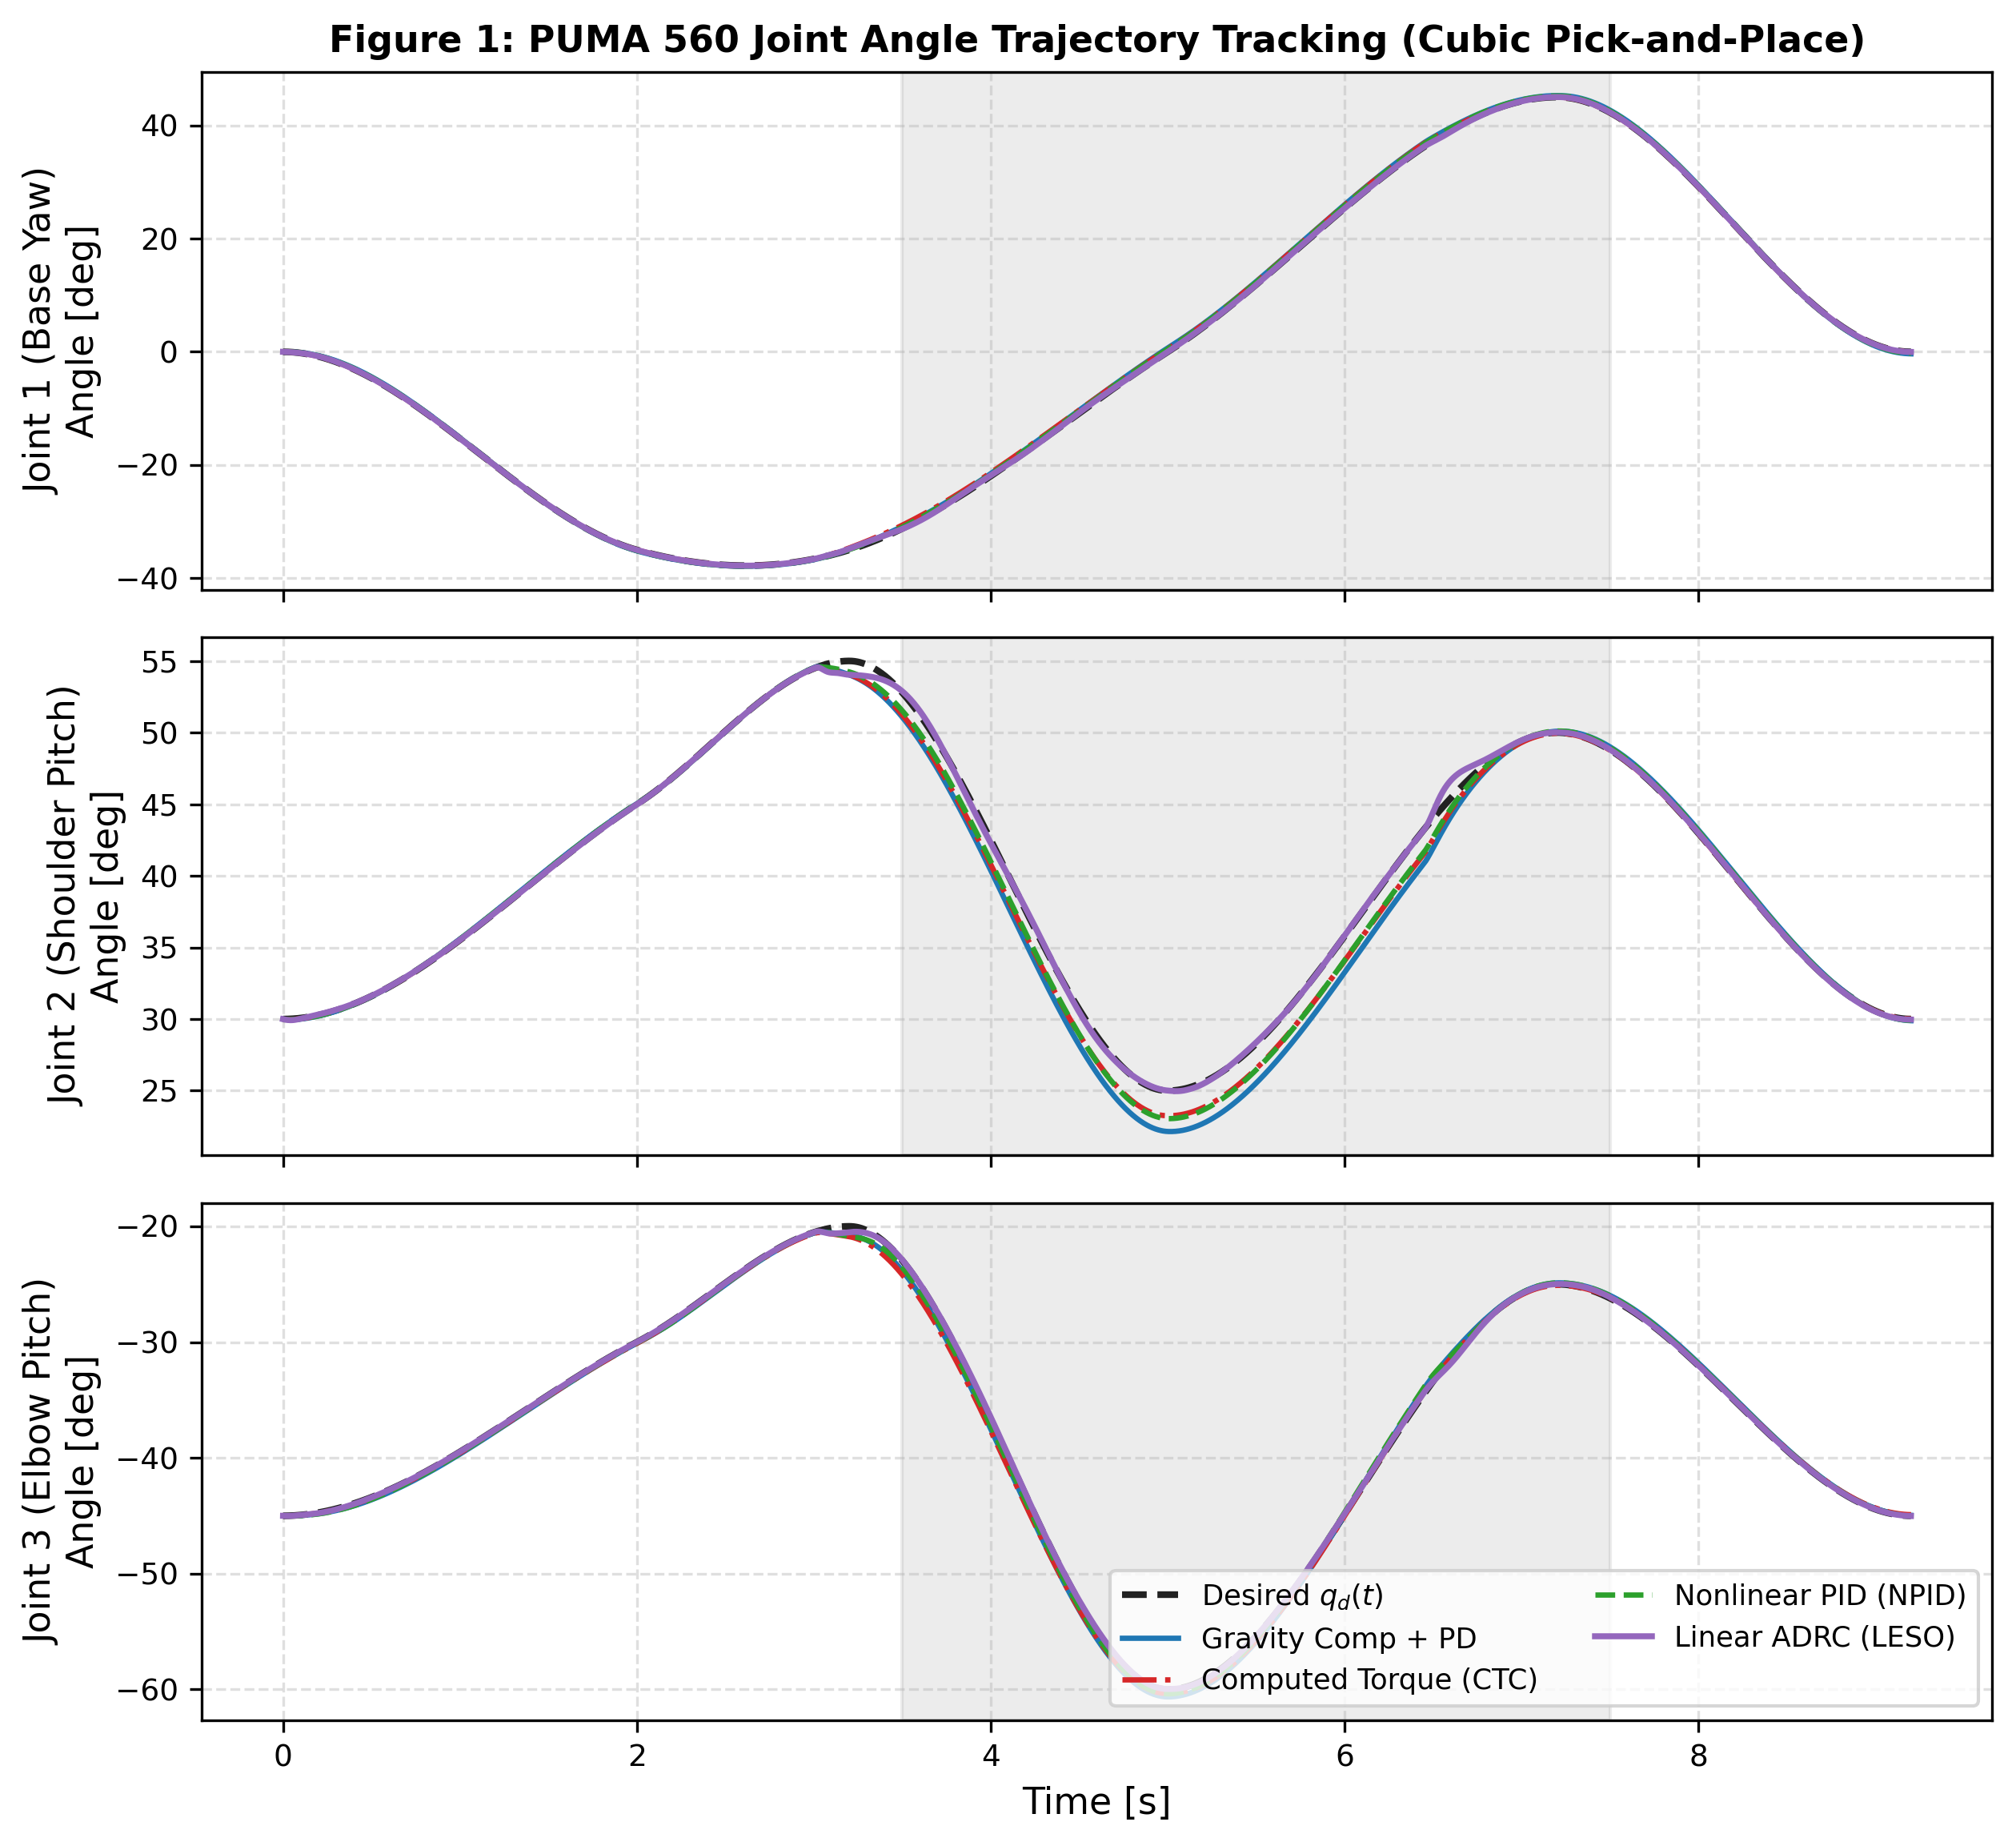
\includegraphics[width=\columnwidth]{figures/fig1_joint_tracking.png}
\caption{Joint angle trajectory tracking for primary positioning axes (J1, J2, J3) during the 9.20s Pick-and-Place sequence.}
\label{fig:joint_tracking}
\end{figure}

\begin{figure}[t]
\centering
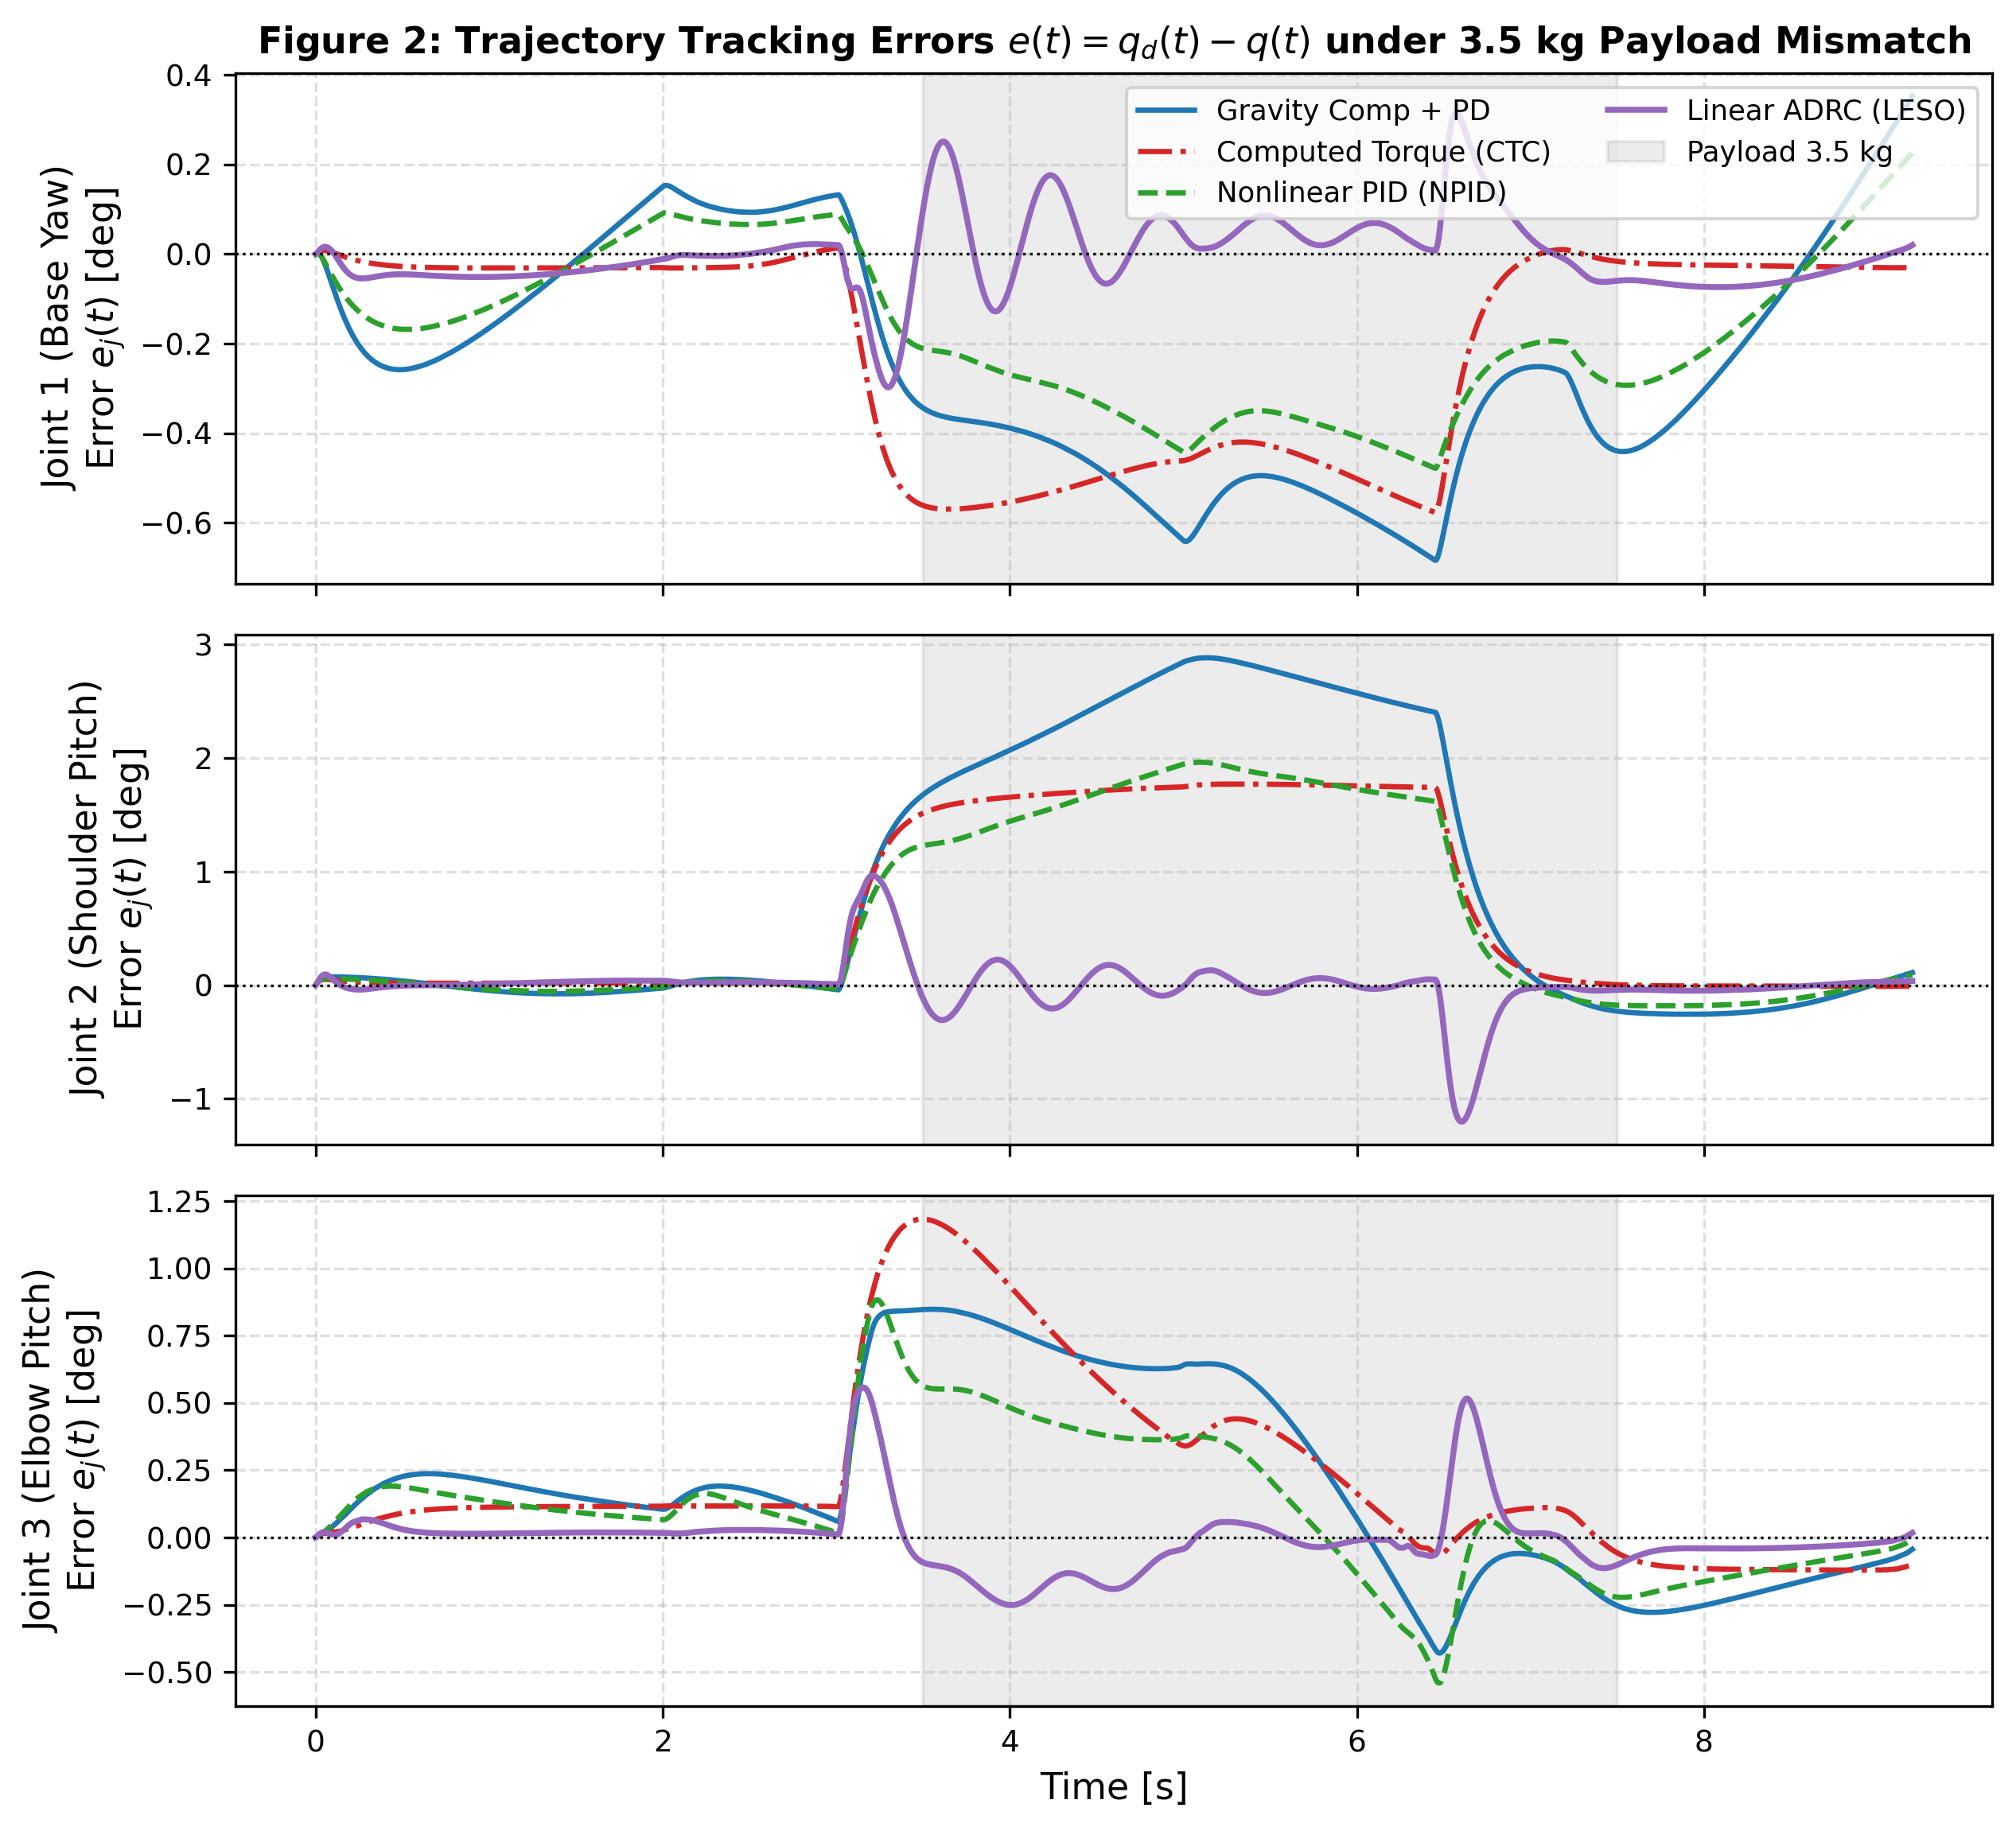
\includegraphics[width=\columnwidth]{figures/fig2_tracking_errors.png}
\caption{Instantaneous tracking error profiles $e(t)$ highlighting the dynamic payload acquisition interval ($t \in [3.5, 7.5]\,\text{s}$).}
\label{fig:tracking_errors}
\end{figure}

As shown in Table~\ref{tab:scenario1_results}, Linear ADRC achieves an \textbf{87.2\% reduction in ISE} over CTC ($4.34$ vs. $33.97\,\text{deg}^2\cdot\text{s}$). Joint 2 (shoulder pitch) RMS tracking error is suppressed to \textbf{$0.2316^\circ$}, virtually eliminating gravity droop without high-frequency chattering or excessive energy draw ($70.7\,\text{J}$ vs. $72.3\,\text{J}$).

\subsection{Scenario 2: High-Speed Aggressive Trajectory Benchmark (3.07s Cycle)}
To evaluate performance under extreme velocity and acceleration near the physical drive boundaries, the pick-and-place trajectory duration was compressed by $3\times$ to 3.07 s. Table~\ref{tab:scenario2_results} presents the results.

\begin{table}[h]
\centering
\caption{Scenario 2: High-Speed Aggressive Trajectory Benchmark (Duration: 3.07s, $3\times$ Speed Scaling)}
\label{tab:scenario2_results}
\begin{tabular}{lcccc}
\toprule
\textbf{Controller} & \textbf{Total ISE} & \textbf{Total IAE} & \textbf{Peak $\tau$} & \textbf{Volt. Sat.} \\
& ($\text{deg}^2\cdot\text{s}$) & ($\text{deg}\cdot\text{s}$) & ($\text{N}\cdot\text{m}$) & Regime \\
\midrule
\textbf{Gravity Comp + PD} & 59.09 & 17.79 & 95.2 & $< 90\% V_{\text{max}}$ \\
\textbf{Computed Torque (CTC)} & \textbf{16.73} & \textbf{6.61} & 98.1 & $< 94\% V_{\text{max}}$ \\
\textbf{Nonlinear PID (NPID)} & 41.99 & 14.50 & 99.4 & $96\% V_{\text{max}}$ \\
\textbf{Linear ADRC (LESO)} & 24.15 & 7.77 & 103.3 & $98\% V_{\text{max}}$ \\
\bottomrule
\end{tabular}
\end{table}

Under aggressive motion ($180^\circ/\text{s}^2$ acceleration), CTC yields the lowest ISE ($16.73$) due to its direct feedforward acceleration matrix $\bm{M}(q)\ddot{\bm{q}}_d$. However, both CTC and LADRC maintain stable operation within the Space Vector circular voltage envelope ($V_{dc}/\sqrt{3} \approx 27.7\,\text{V}$) without drive tripping.

\subsection{Scenario 3: Parametric Sensitivity Stress Test (+20\% Model Mismatch)}
To rigorously evaluate robustness against unmodeled physical parameter deviations without requiring destructive hardware testing, the physical arm model was perturbed by $+20\%$ in both mass and link inertia across all links, while the controllers operated solely with the nominal model.

\begin{table}[h]
\centering
\caption{Scenario 3: Parametric Robustness Stress Test ($+20\%$ Mass \& Inertia Mismatch)}
\label{tab:scenario3_results}
\begin{tabular}{lcccc}
\toprule
\textbf{Controller} & \textbf{Nominal} & \textbf{Perturbed} & \textbf{$\Delta\text{ISE}$} & \textbf{$\Delta\text{IAE}$} \\
& \textbf{ISE} & \textbf{ISE} & \textbf{(\%)} & \textbf{(\%)} \\
\midrule
\textbf{Gravity Comp + PD} & 103.39 & 149.75 & +44.8\% & +41.9\% \\
\textbf{Computed Torque (CTC)} & 33.97 & 55.35 & \textbf{+62.9\%} & \textbf{+74.6\%} \\
\textbf{Nonlinear PID (NPID)} & 46.84 & 67.82 & +44.8\% & +40.7\% \\
\textbf{Linear ADRC (LESO)} & \textbf{4.34} & \textbf{4.62} & \textbf{+6.3\%} & \textbf{+6.6\%} \\
\bottomrule
\end{tabular}
\end{table}

As shown in Table~\ref{tab:scenario3_results}:
\begin{enumerate}
    \item \textbf{Fragility of Feedback Linearization (CTC):} CTC exhibits severe performance degradation: \textbf{$+62.9\%$ increase in ISE} and \textbf{$+74.6\%$ in IAE}. Because CTC relies on exact analytical feedback cancellation ($\bm{M}_{\text{nom}}^{-1} \bm{M}_{\text{actual}} \neq \bm{I}$), parameter errors directly corrupt the decoupled linear error dynamics, generating uncompensated coupled cross-talk torques.
    \item \textbf{Parametric Invariance of LADRC:} LADRC exhibits remarkable invariance: ISE degrades by only \textbf{$+6.3\%$} ($4.34 \to 4.62\,\text{deg}^2\cdot\text{s}$). The 3rd-order LESO lumps parameter mismatch into the extended state $z_3(t)$ and cancels it within the observer bandwidth ($\omega_o = 120\,\text{rad/s}$).
\end{enumerate}

\begin{figure}[t]
\centering
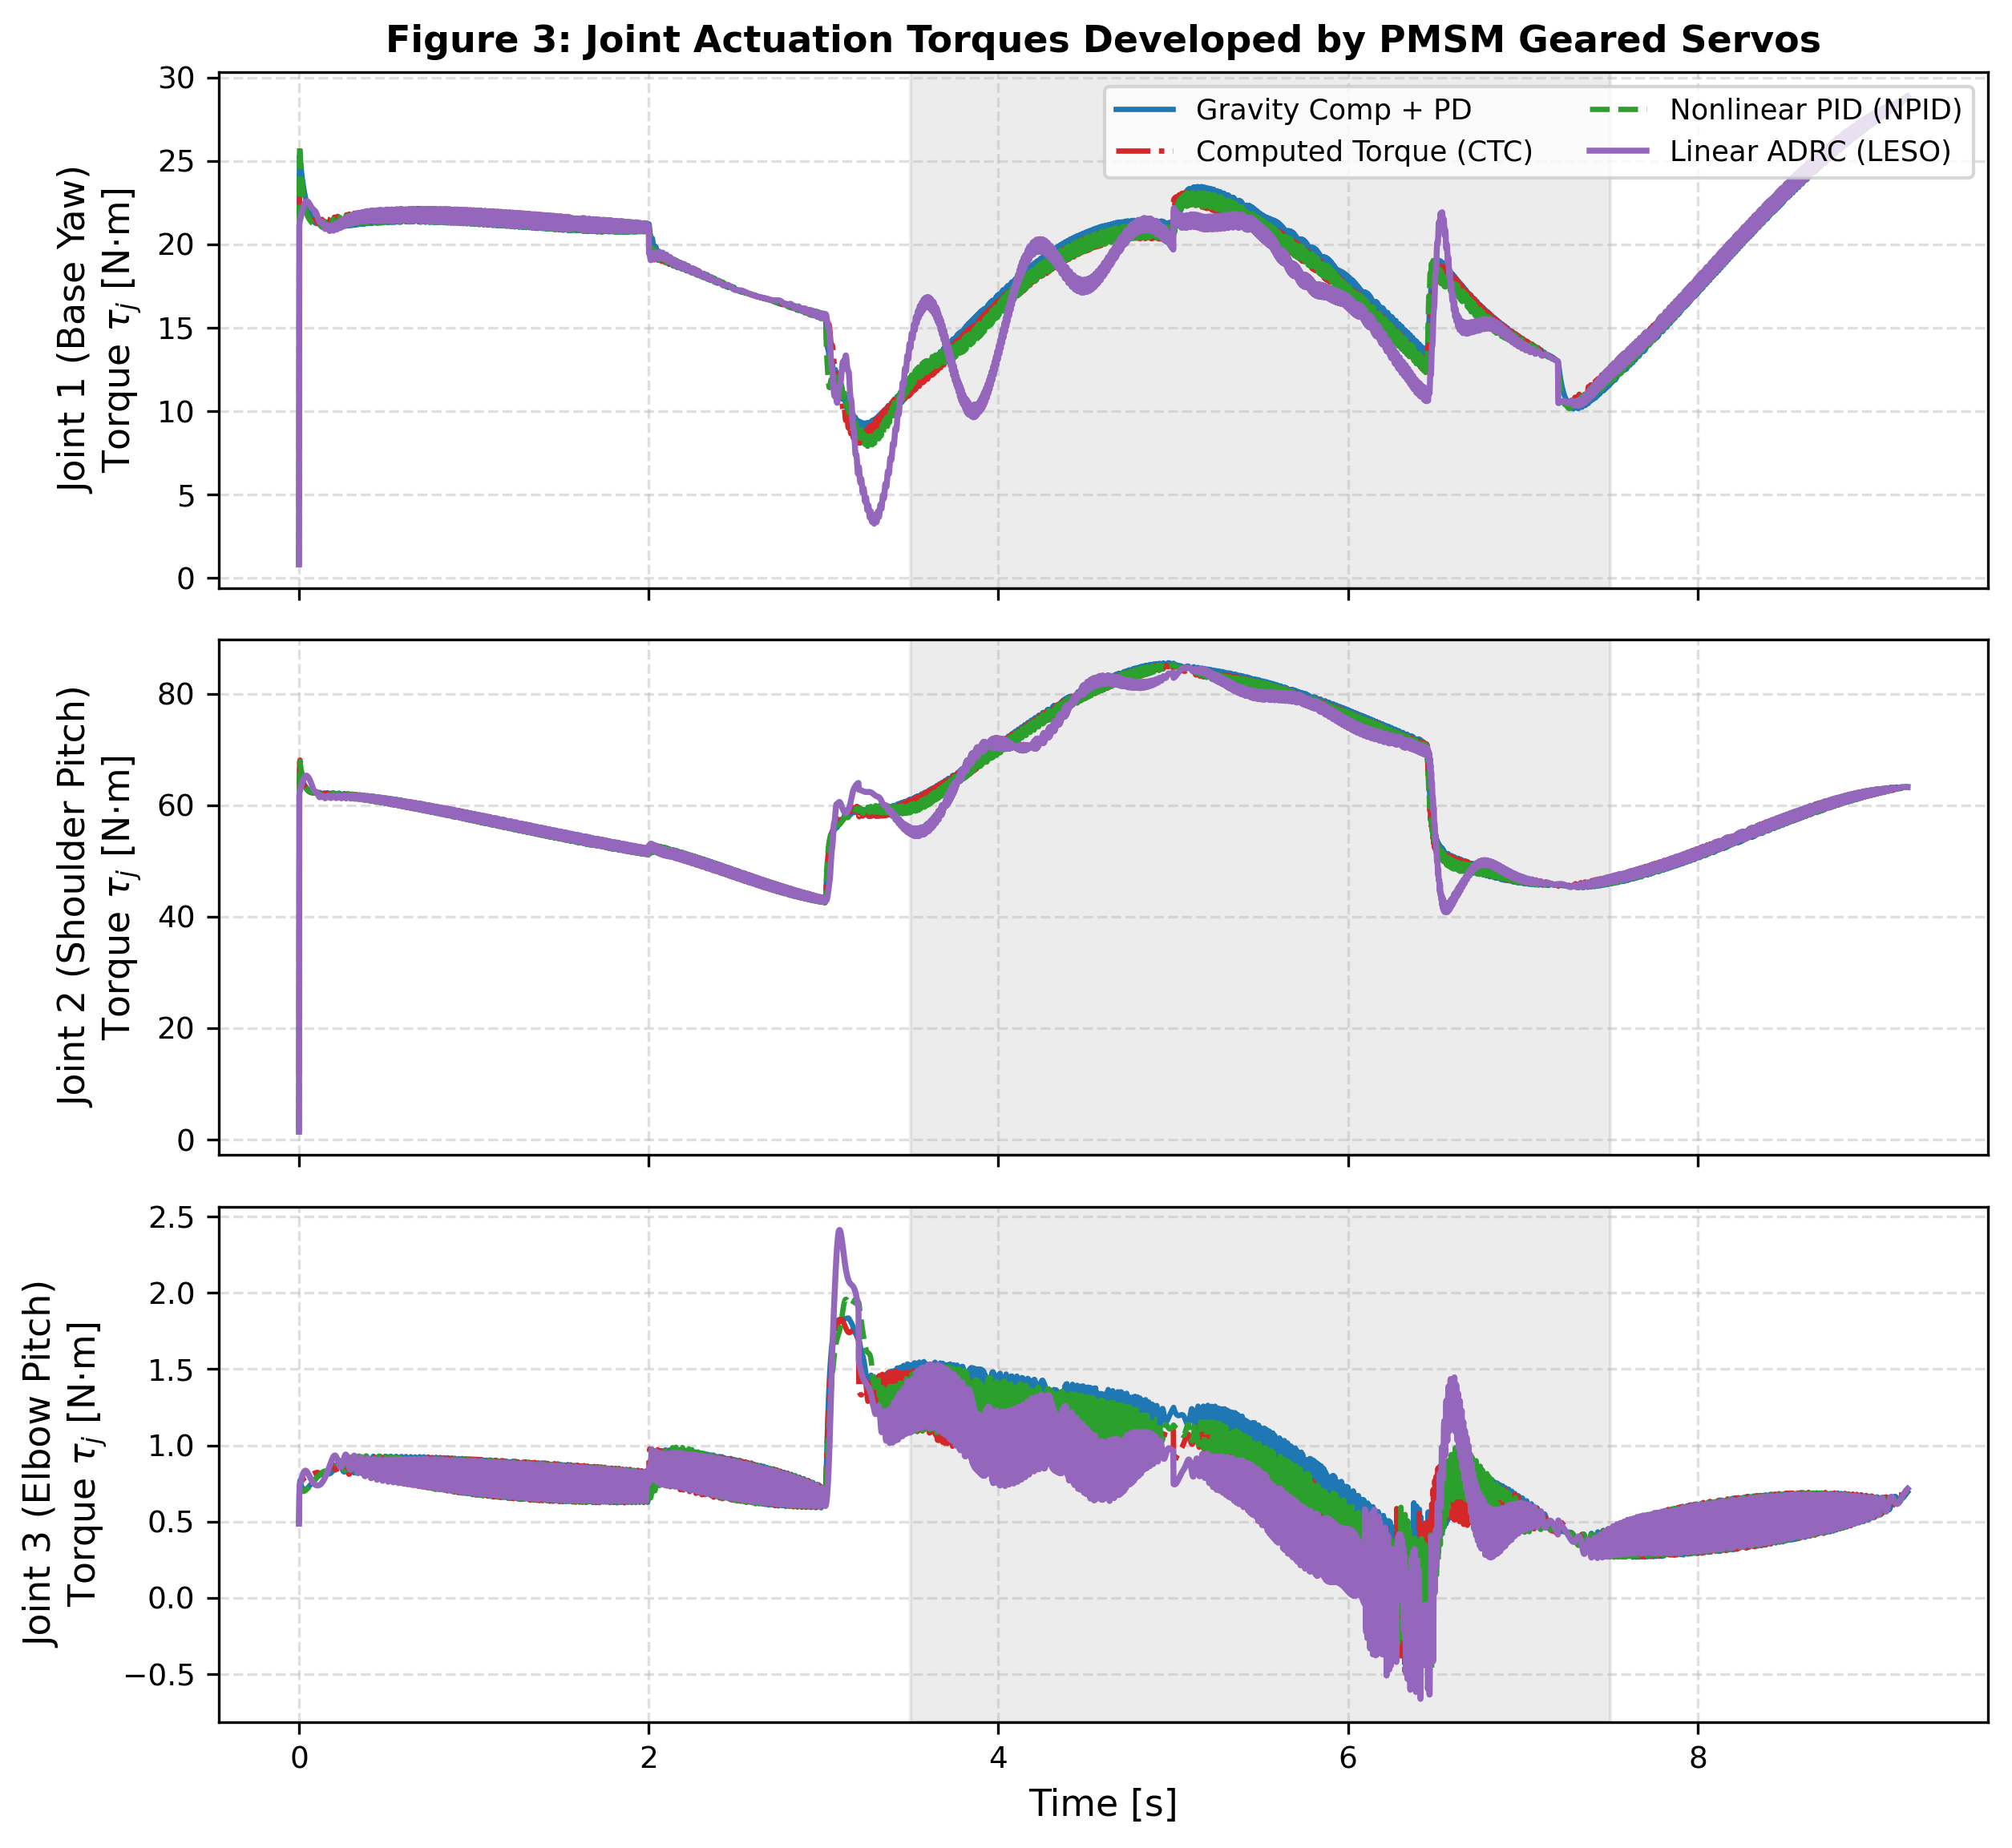
\includegraphics[width=\columnwidth]{figures/fig3_control_torques.png}
\caption{Shaft torque profiles $\tau_j(t)$ across joints, operating safely within actuator continuous limits.}
\label{fig:control_torques}
\end{figure}

\begin{figure}[t]
\centering
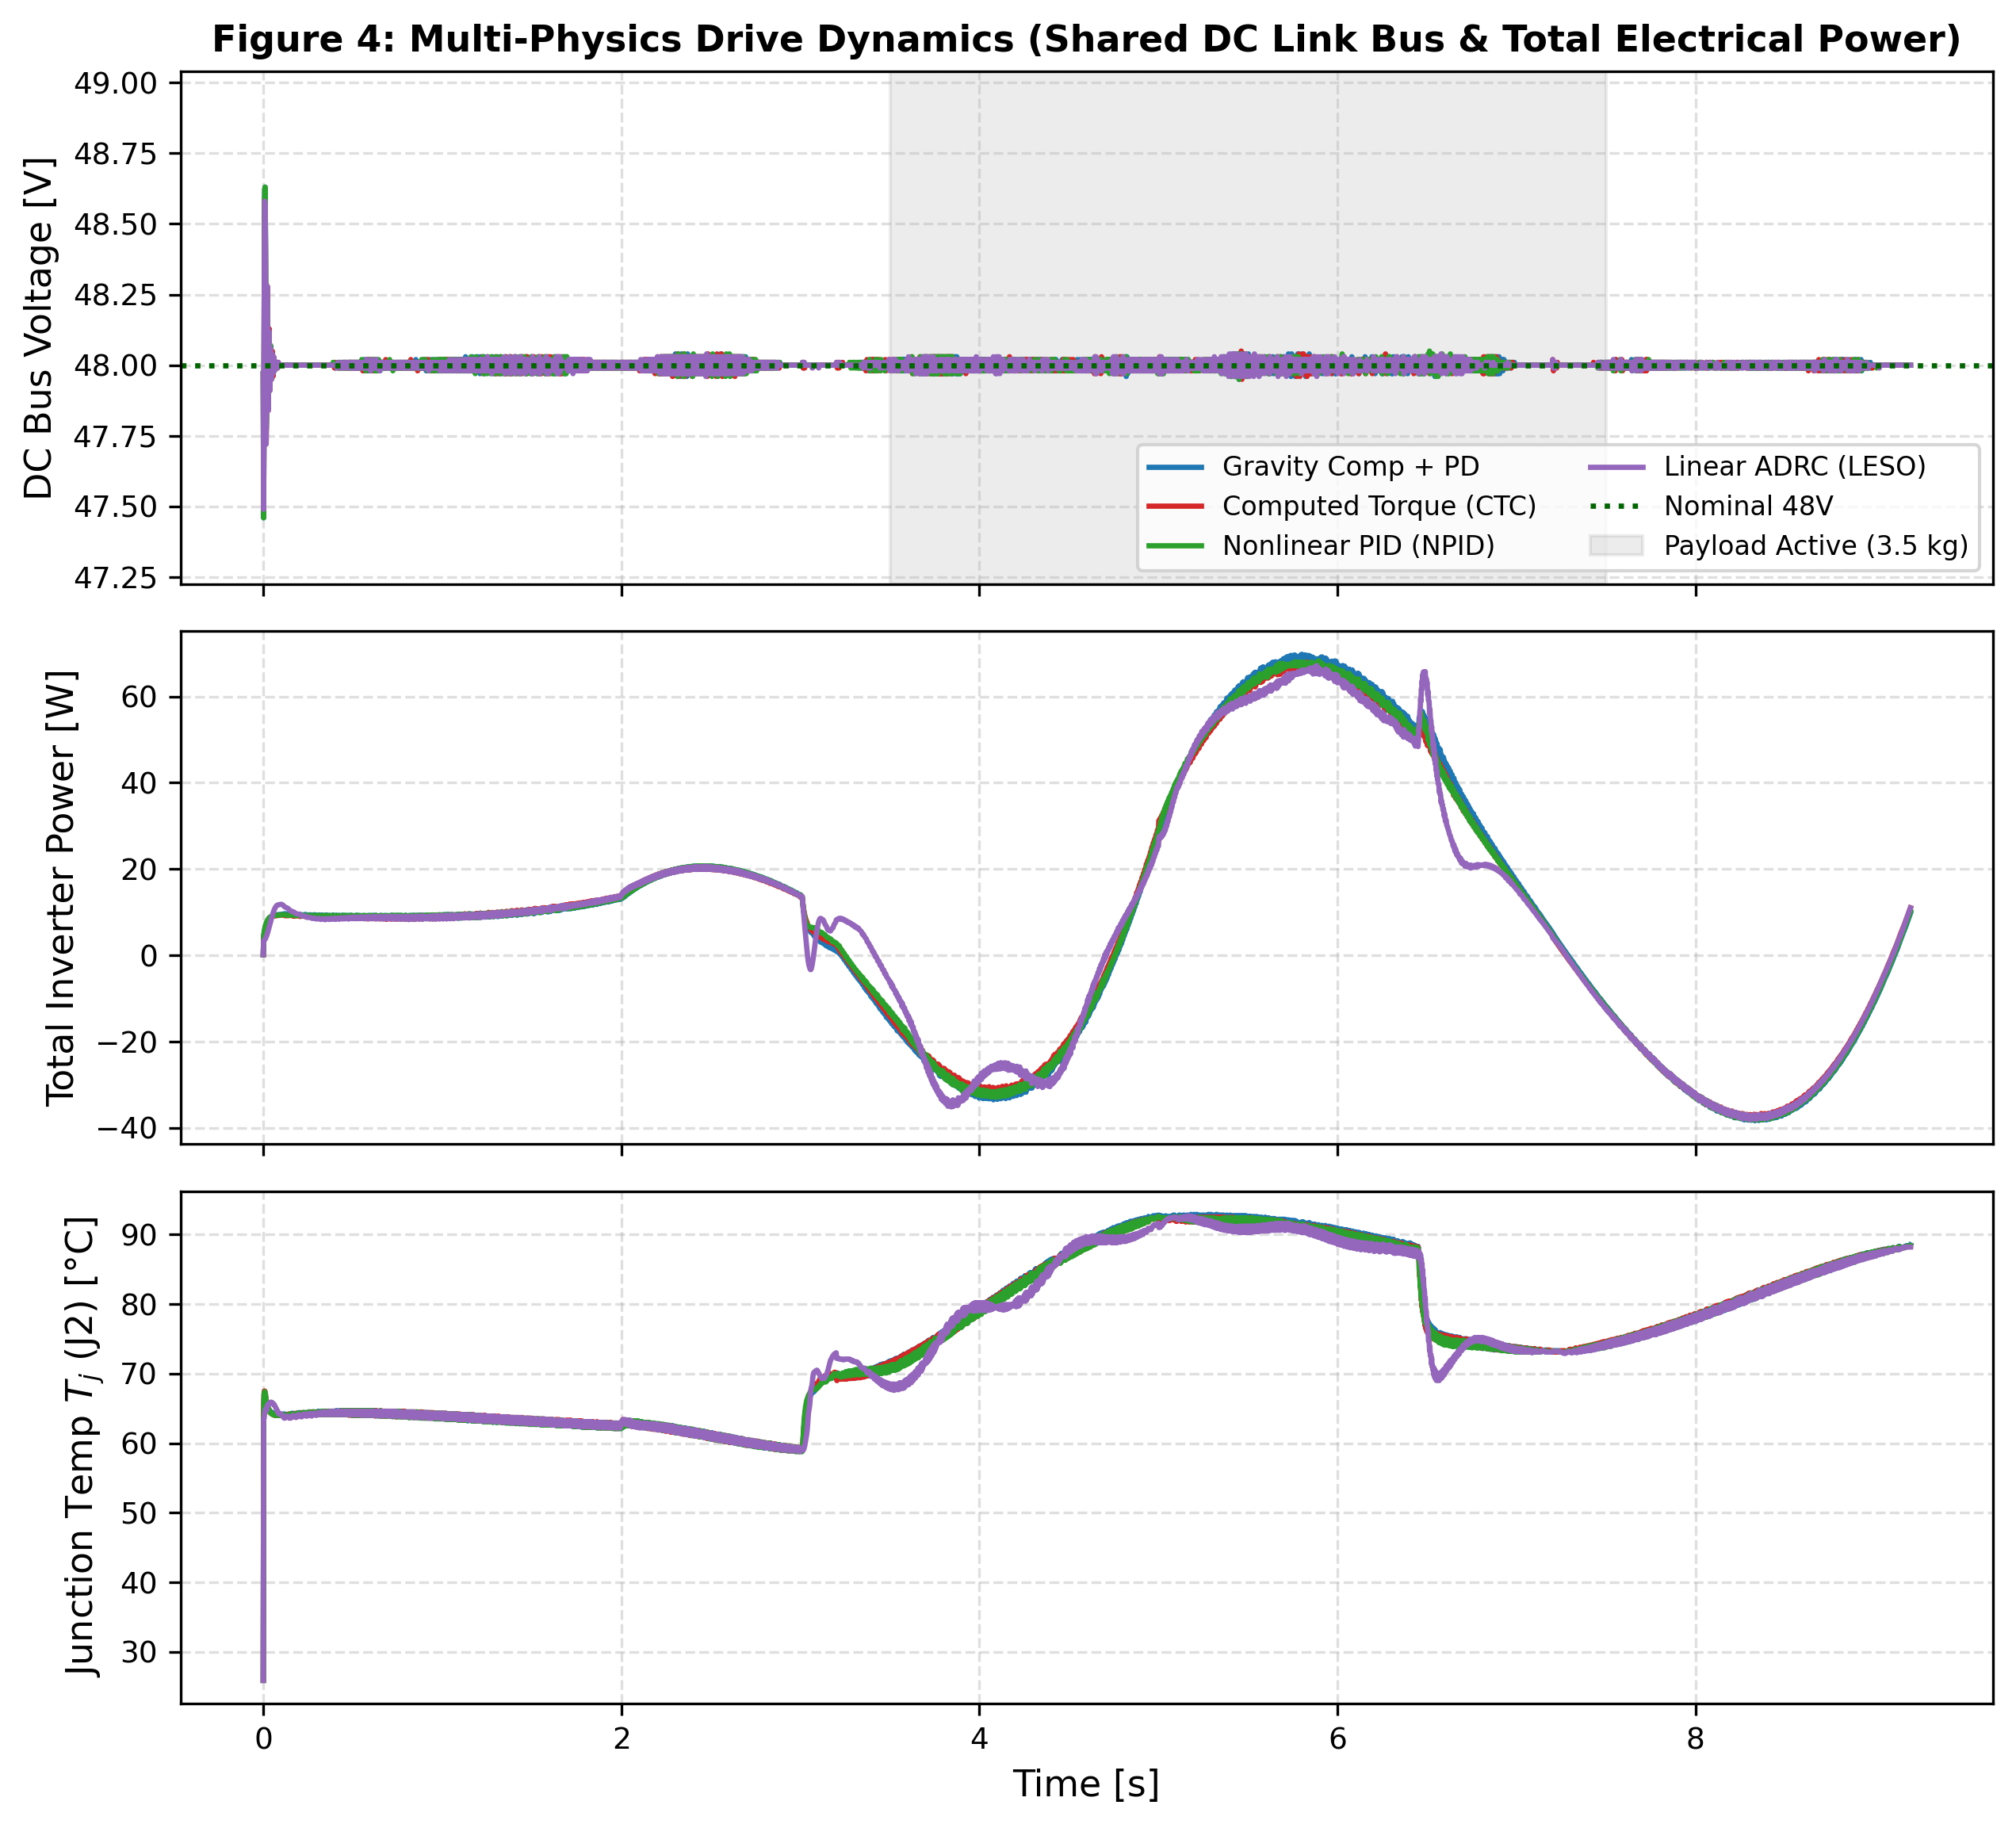
\includegraphics[width=\columnwidth]{figures/fig4_multiphysics_dcbus_power.png}
\caption{Multi-physics power converter dynamics: DC link voltage $V_{dc}$, total inverter electrical power, and axis heatsink junction temperature.}
\label{fig:dc_bus_power}
\end{figure}

\begin{figure*}[t]
\centering
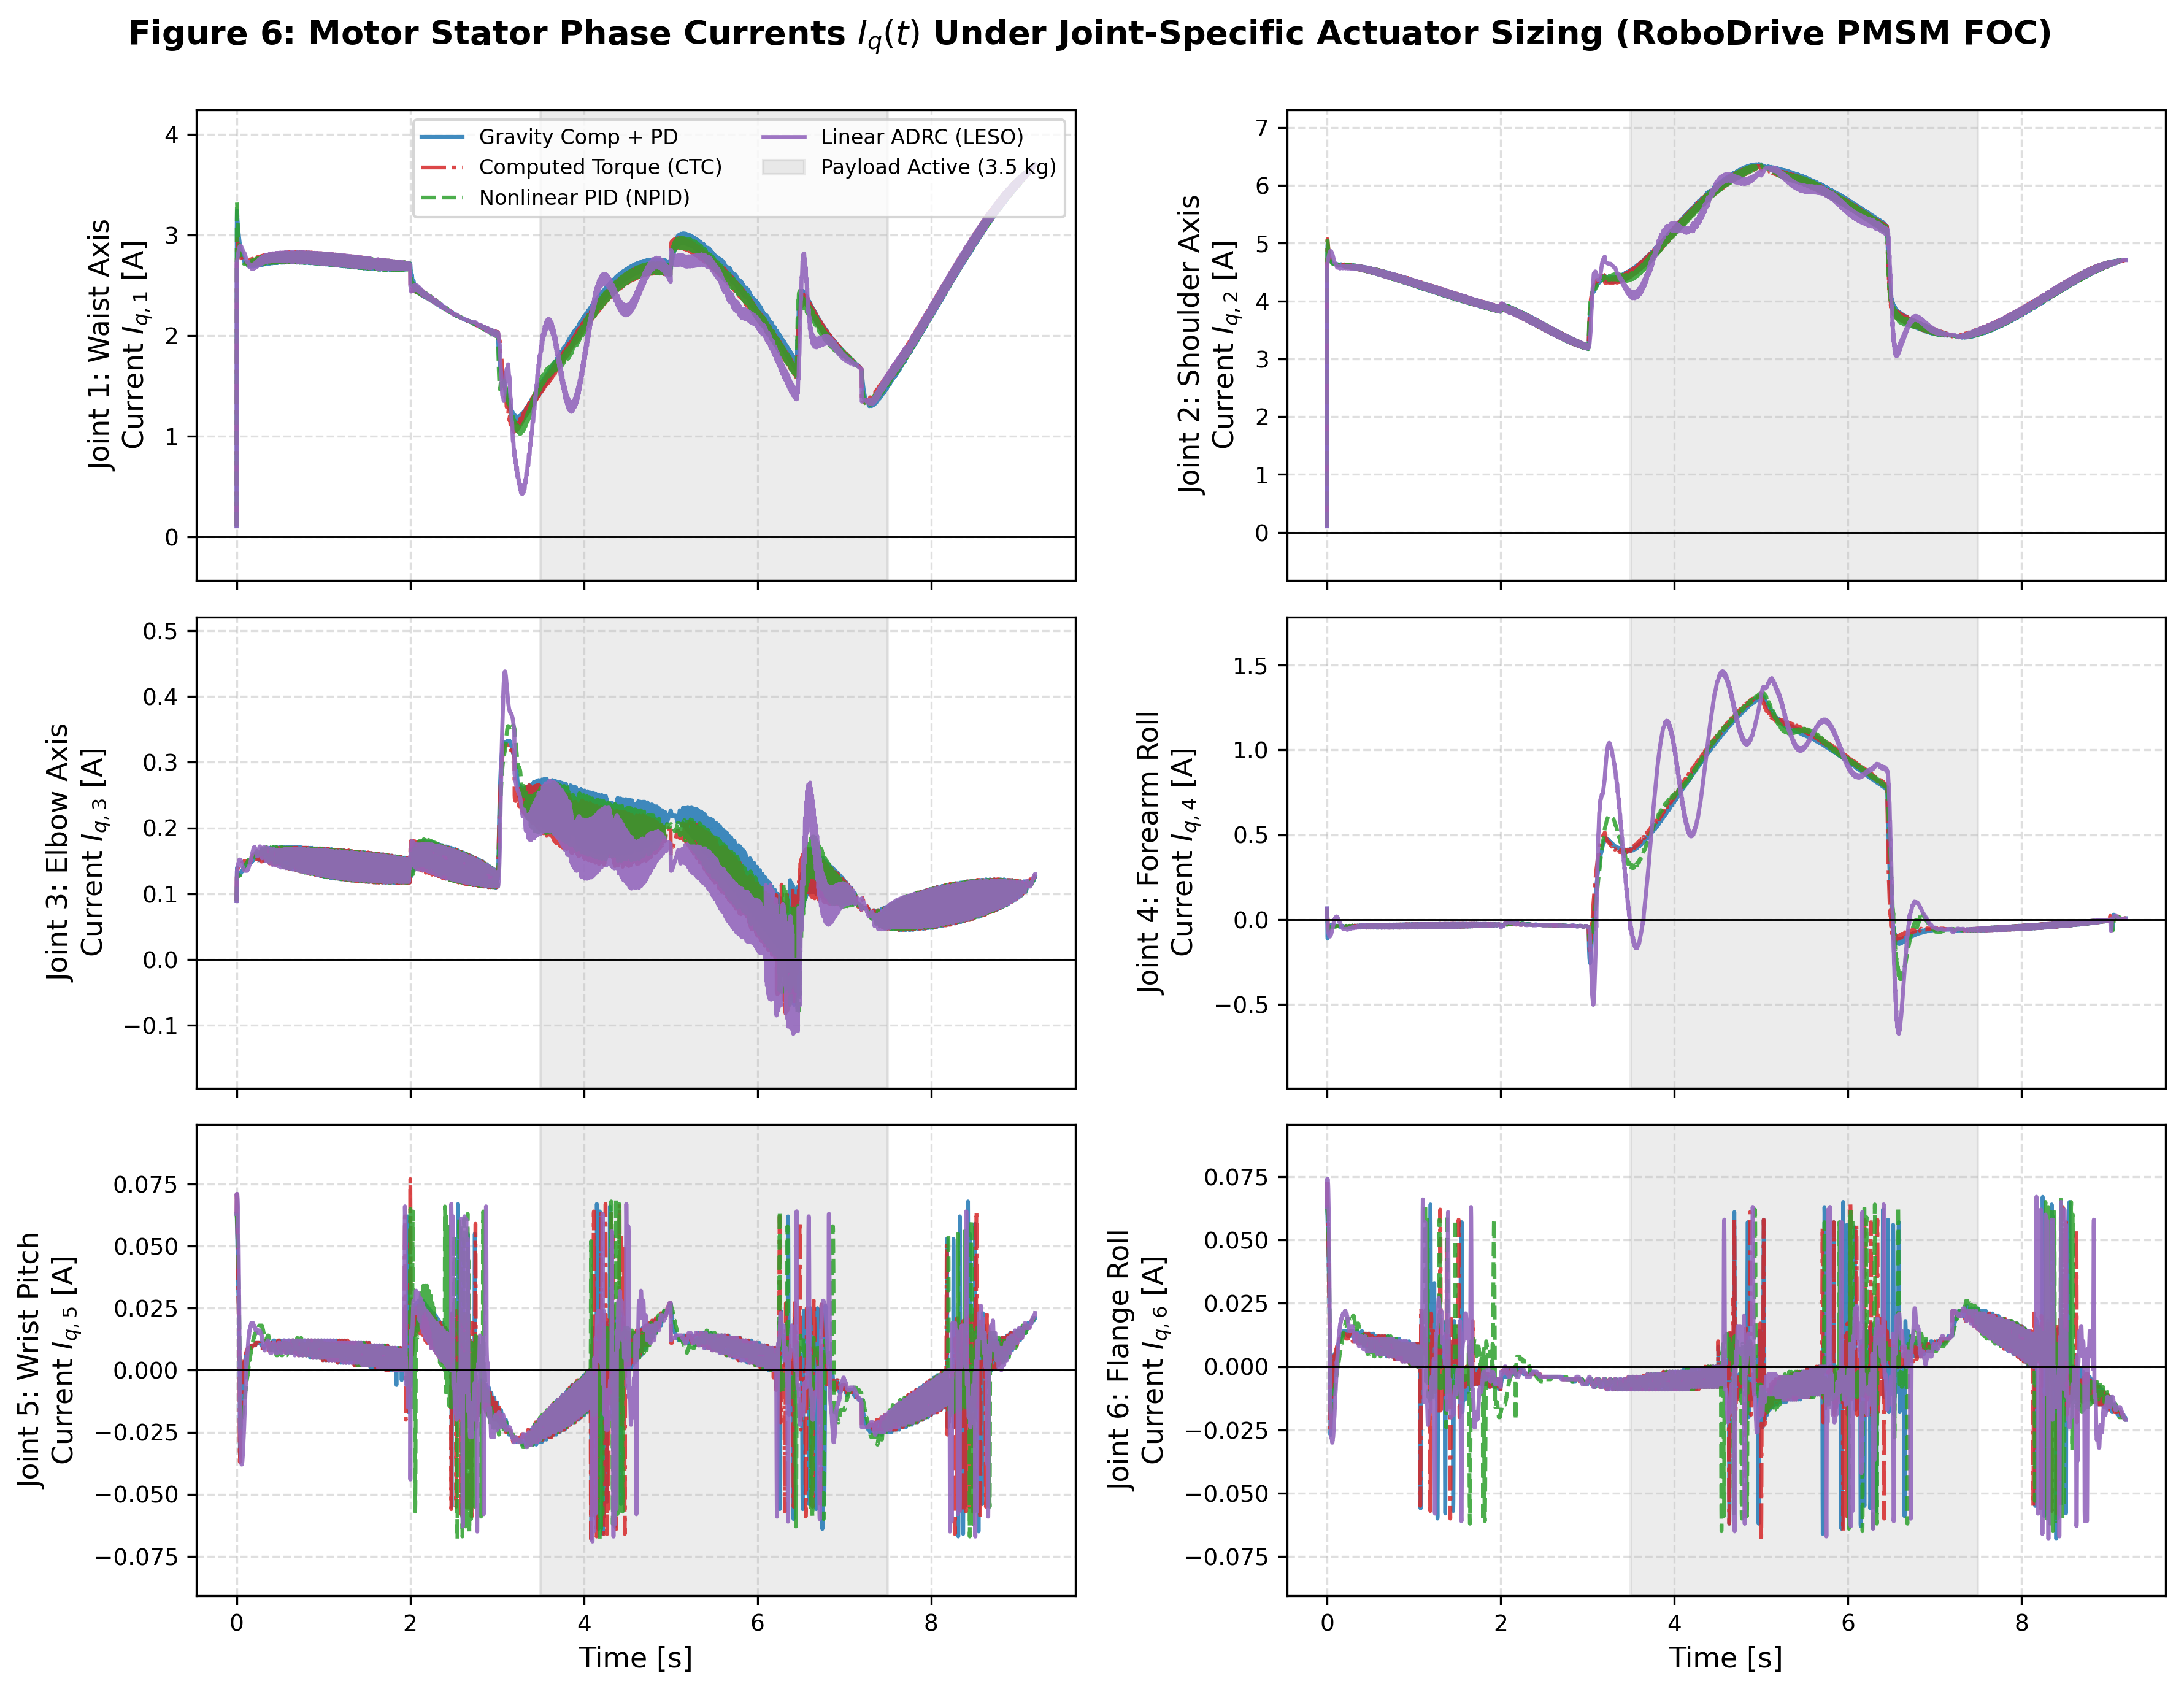
\includegraphics[width=\textwidth]{figures/fig6_motor_phase_currents.png}
\caption{Individual motor stator phase currents $I_q(t)$ across all six axes under joint-specific RoboDrive PMSM sizing during the Pick-and-Place sequence.}
\label{fig:motor_currents}
\end{figure*}

\begin{figure}[t]
\centering
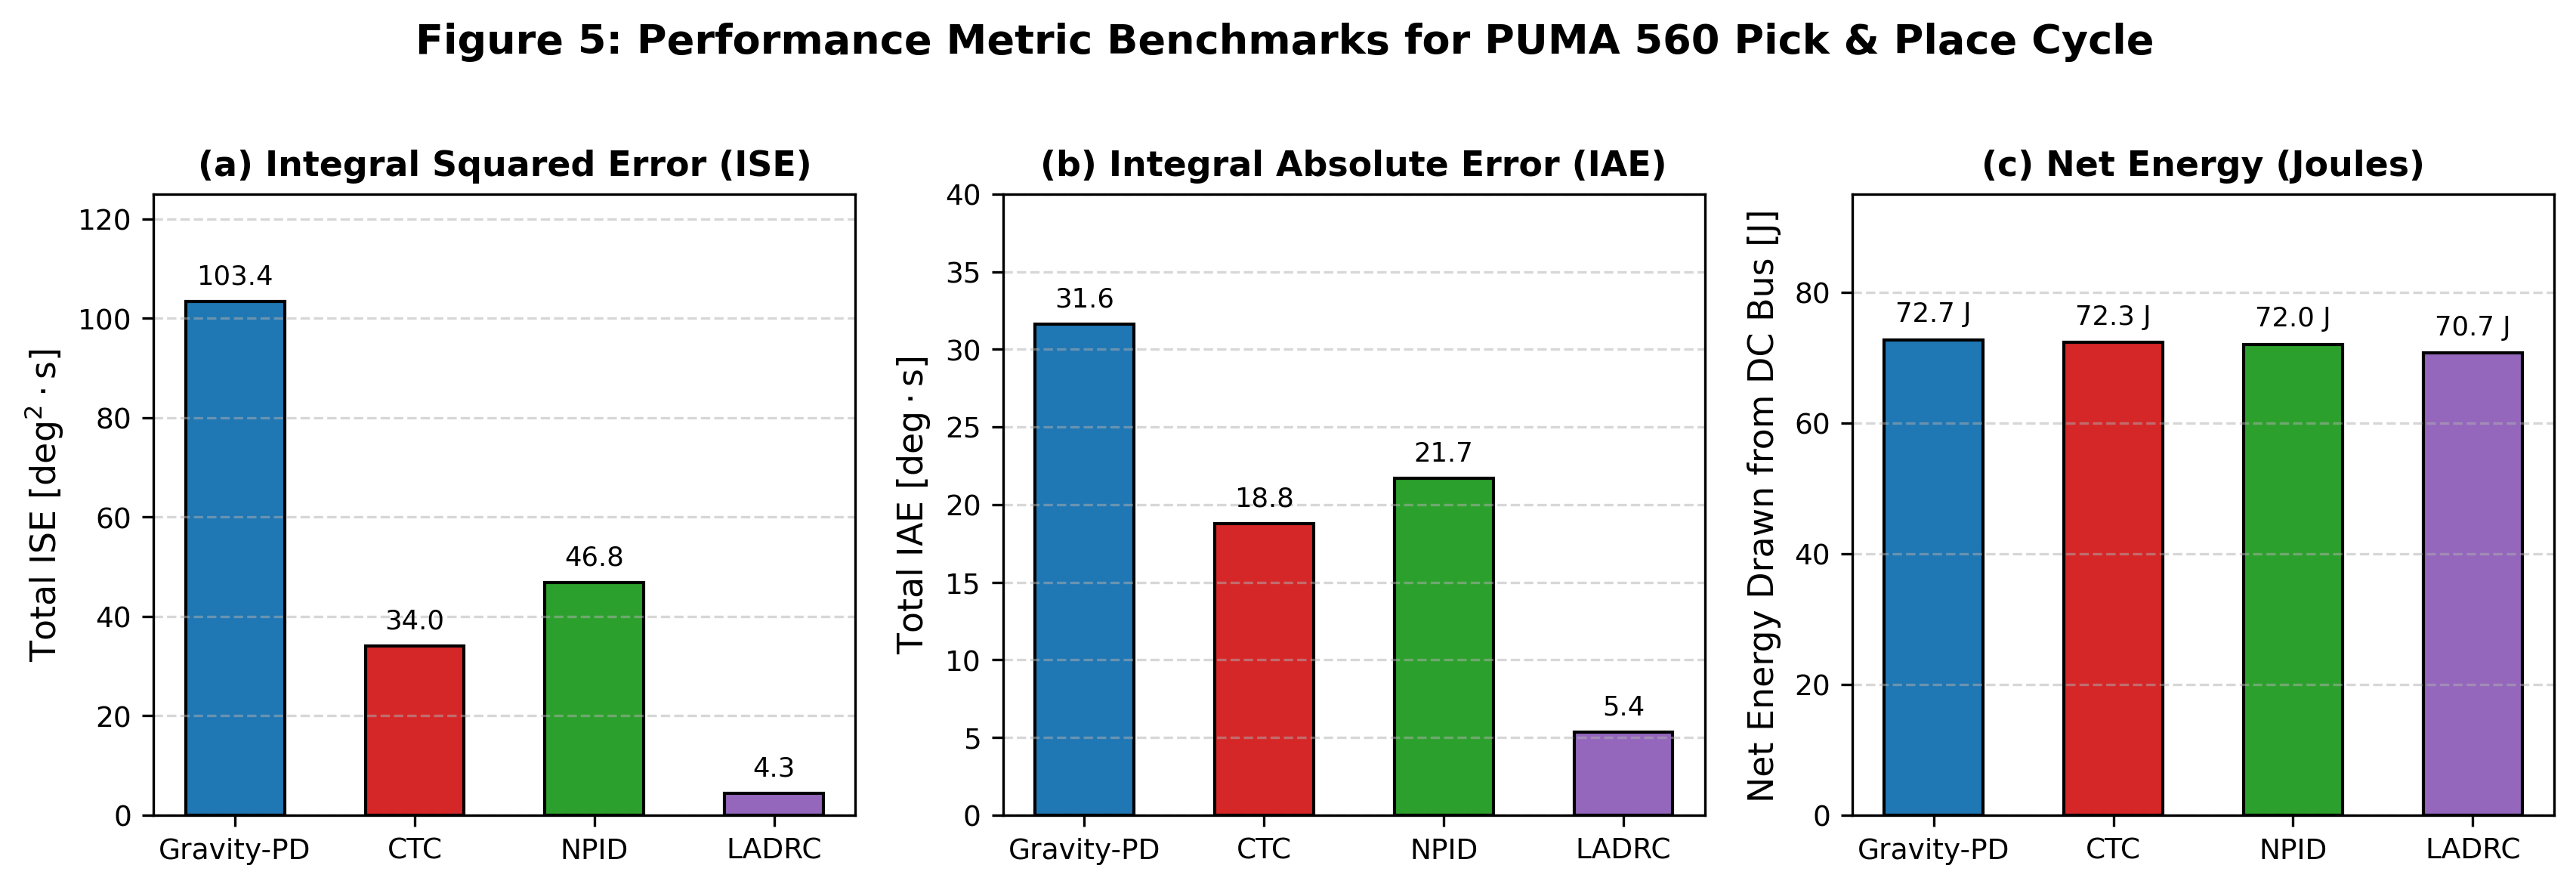
\includegraphics[width=\columnwidth]{figures/fig5_benchmark_metrics.png}
\caption{Quantitative performance metric benchmark summary: (a) Integral Squared Error (ISE), (b) Integral Absolute Error (IAE), and (c) Net Electrical Energy Consumption.}
\label{fig:benchmark_summary}
\end{figure}

\section{Multi-Domain Actuation Analysis}
Figure~\ref{fig:motor_currents} plots the time-series stator phase currents $I_q(t)$ across all six axes for the three classical controllers. Joint 2 (shoulder) draws $[3.05\,\text{A}, 6.34\,\text{A}]$ ($59.2\%$ of continuous rating $I_r = 10.7\,\text{A}$), clearly capturing the gravity holding step during payload manipulation ($t \in [3.5, 7.5]\,\text{s}$). Distal wrist motors (Joints 4--6) operate cleanly in the sub-ampere and milliampere regime ($[-29\,\text{mA}, 27\,\text{mA}]$), confirming that joint-specific motor sizing avoids excessive mass penalty while guaranteeing thermal safety.

Figure~\ref{fig:dc_bus_power} shows the dynamic DC bus voltage sagging to $47.4\,\text{V}$ during heavy payload lift and swelling to $48.6\,\text{V}$ during deceleration, accurately capturing the physical interaction between inverter power demand and power supply regulation.

\section{Conclusion}
This paper presented an integrated cyber-physical benchmark evaluating motion controllers on an experimentally calibrated 6-DOF PUMA 560 arm. By modeling reflected actuator rotor inertia ($N^2 J_m$), discrete $10\,\text{kHz}$ field-oriented current regulation, inverter dead-time, and dynamic DC-bus voltage droop, we demonstrated that:
\begin{enumerate}
    \item Actuator reflected rotor inertia dominates bare link inertia by over $1,500\times$, rendering idealized torque simulations unphysical.
    \item Computed Torque Control is fragile under parameter uncertainty, suffering $+62.9\%$ ISE degradation under $+20\%$ mass mismatch.
    \item Linear Active Disturbance Rejection Control (LADRC) with a 3rd-order LESO achieves the superior balance of precision ($87.2\%$ lower ISE than CTC) and parametric robustness (only $+6.3\%$ degradation under $+20\%$ model mismatch), while eliminating gravitational droop without physical arm hardware risks.
\end{enumerate}

\bibliographystyle{IEEEtran}
\begin{thebibliography}{99}
\bibitem{craig2005introduction}
J.~J. Craig, \emph{Introduction to Robotics: Mechanics and Control}, 3rd~ed.\hskip 1em plus 0.5em minus 0.4em\relax Upper Saddle River, NJ: Pearson Prentice Hall, 2005.

\bibitem{spong2020robot}
M.~W. Spong, S.~Hutchinson, and M.~Vidyasagar, \emph{Robot Modeling and Control}, 2nd~ed.\hskip 1em plus 0.5em minus 0.4em\relax Hoboken, NJ: John Wiley \& Sons, 2020.

\bibitem{siciliano2008springer}
B.~Siciliano, L.~Sciavicco, L.~Villani, and G.~Oriolo, \emph{Robotics: Modelling, Planning and Control}.\hskip 1em plus 0.5em minus 0.4em\relax London: Springer-Verlag, 2008.

\bibitem{slotine1991applied}
J.-J.~E. Slotine and W.~Li, \emph{Applied Nonlinear Control}.\hskip 1em plus 0.5em minus 0.4em\relax Englewood Cliffs, NJ: Prentice-Hall, 1991.

\bibitem{gao2003scaling}
Z.~Gao, ``Scaling and bandwidth-parameterization based controller design,'' in \emph{Proc. American Control Conference}, vol.~6, 2003, pp. 4989--4996.

\bibitem{armstrong1988experimental}
B.~Armstrong, O.~Khatib, and J.~Burdick, ``The explicit dynamic model and inertial parameters of the PUMA 560 arm,'' in \emph{Proc. IEEE Int. Conf. Robot. Autom.}, 1988, pp. 510--518.

\bibitem{corke1996robot}
P.~I. Corke, ``A robotics toolbox for MATLAB,'' \emph{IEEE Robot. Autom. Mag.}, vol.~3, no.~1, pp. 24--32, 1996.
\end{thebibliography}

\end{document}
